%! TEX root = ../main.tex
\documentclass[../main.tex]{subfiles}

\begin{document}

\section{Risultati}

Avendo preso le misure a partire da un'estremità della guida dentata la curva non ha il picco centrato in $y = 0$, quindi si è proceduto con il traslare le misure. L'errore attribuito a questa operazione è di $\qty{1}{\mm}$.

A partire dai dati raccolti con apertura del sensore pari a $\qty{1.5}{\mm}$ 
è stata stimata la dimensione della fenditura utilizzando due metodi

\begin{enumerate}
    \item La posizione dei minimi ricavata graficamente che permette di ottenere la dimensione della fenditura utilizzando l'\autoref{eq:y=0 values}
    \item Il fit tramite l'\autoref{eq:fit}, in cui è stato inserito un parametro $c$ che permette di traslare la curva verticalmente in modo da tenere in considerazione la presenza di rumore.
\end{enumerate}

\begin{equation} \label{eq:fit}
    I(I_{0}, a, c) = I_{0} \; \sinc^{2} \left( \frac{\pi a}{\lambda} \cdot \frac{y}{L} \right) + c
\end{equation}

\subsection{Fenditura $a = \qty{0.02}{\milli\metre}$}

\begin{figure}[ht!]
    \centering
    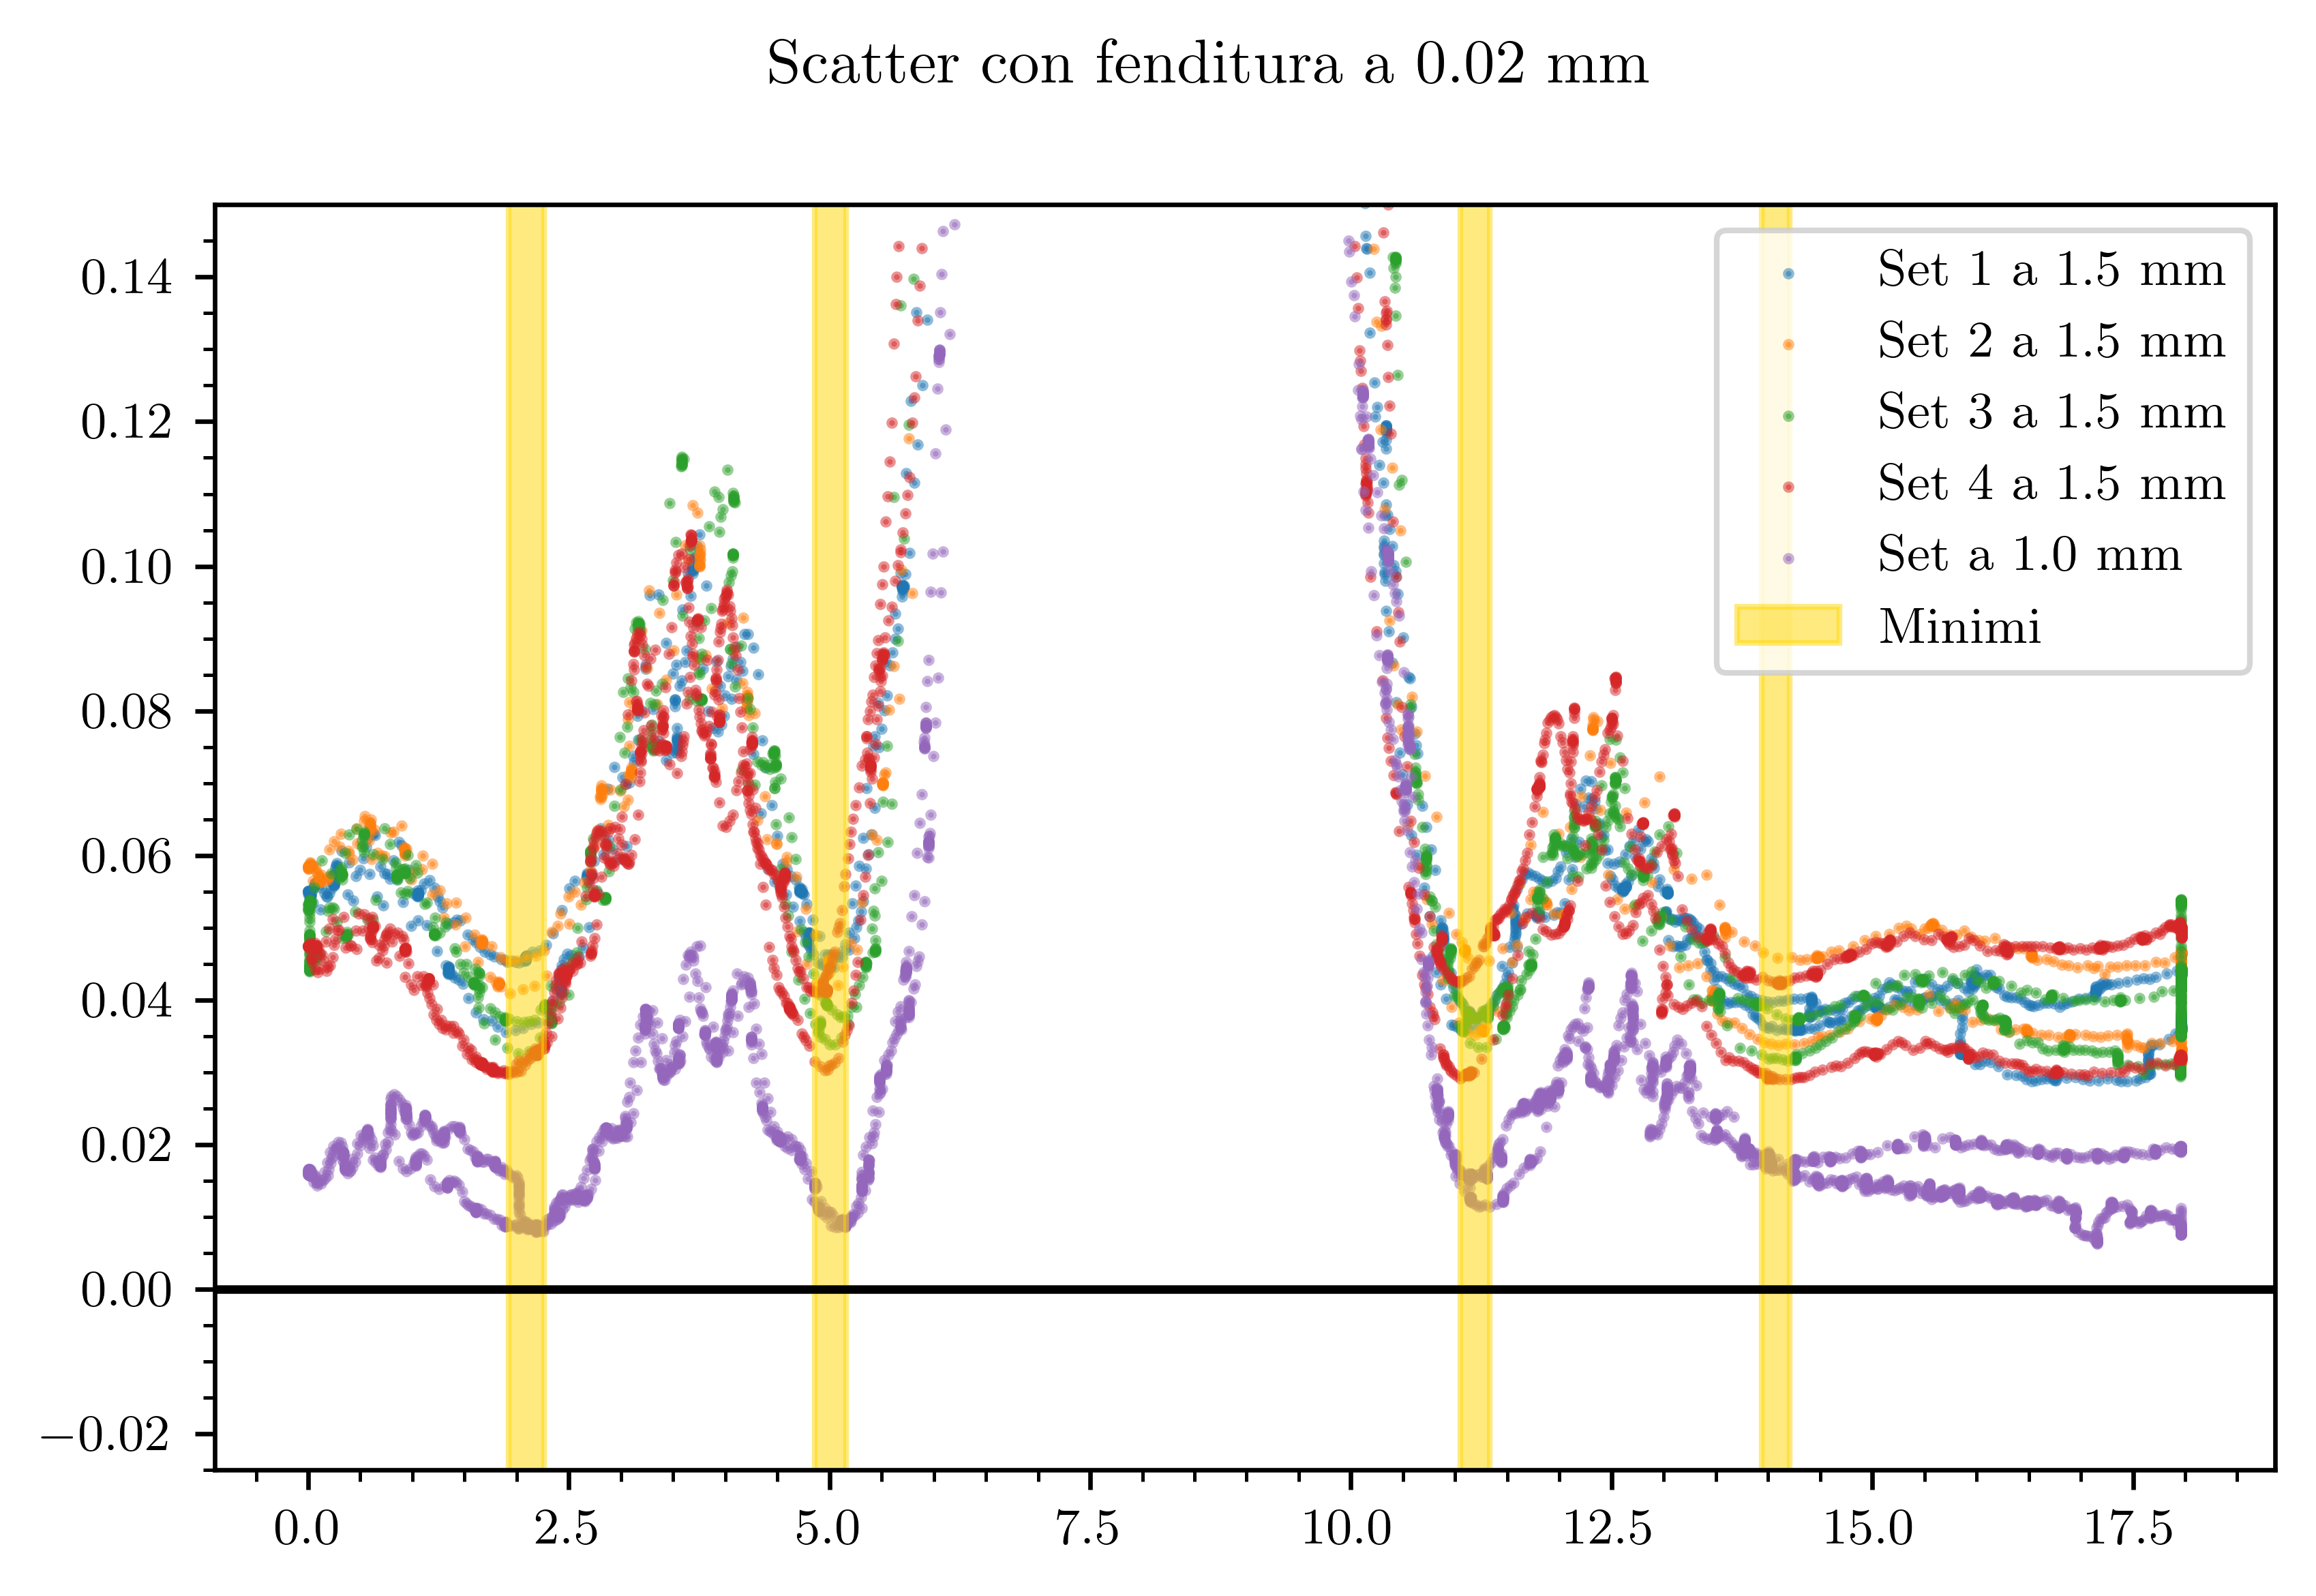
\includegraphics{min_0.02.png}
    \caption{Intensità luminosa $I$ in funzione della posizione $y$ del sensore (in metri) per la fenditura a $\qty{0.02}{\milli\metre}$. In figura sono segnati i minimi ricavati graficamente con i relativi errori. È possibile notare un segnale a frequenza costante che si sovrappone alla figura di diffrazione.} % todo: aggiungere qualcosa in più alla descrizione
    \label{fig:minimi 0.02}
\end{figure}

Le ascisse ottenute dei minimi sono le seguenti:

\begin{table}[ht!]
    \centering
    \caption{Posizione dei minimi, ottenuta graficamente dalla \autoref{fig:minimi 0.02}, riportata di fianco al proprio indice $m$ ed al valore $\frac{\lambda L}{a} \; (\si{\metre})$ stimati seguendo l'\autoref{eq:y=0 values}. Il valore di $a$ derivato da ciascun minimo è stato ricavato con la formula inversa dopo aver posto $\lambda = \qty{650}{\nm}$ ed $L = \qty{98.5}{\cm}$.}
    \begin{tabular}{r|cc|c}
        \toprule
        $m$  & $y \; (\si{\metre})$ & $\frac{\lambda L}{a} \; (\si{\metre})$ & $a \; (\si{\mm})$ \\
        \midrule
        $-2$ & $-0.0613 \pm 0.0013$ & $0.0307 \pm 0.0007$ & \num{0.0209+-0.0005} \\
        $-1$ & $-0.0313 \pm 0.0013$ & $0.0313 \pm 0.0013$ & \num{0.0205+-0.0009} \\
        $1$  & $0.0304 \pm 0.0014$  & $0.0304 \pm 0.0014$ & \num{0.0211+-0.0010} \\
        $2$  & $0.0610 \pm 0.0018$  & $0.0305 \pm 0.0009$ & \num{0.0210+-0.0006} \\
        \bottomrule
    \end{tabular}
    \label{tab:minimi 0.02}
\end{table}

Facendo una media dei valori ricavati 

\subsection{Fenditura $a = \qty{0.04}{\milli\metre}$}



\subsection{Fenditura $a = \qty{0.08}{\milli\metre}$}



%... Per i 4 grafici seguenti, è stata utilizzata la sensibilità "candela".

% \begin{figure}[ht!]
%     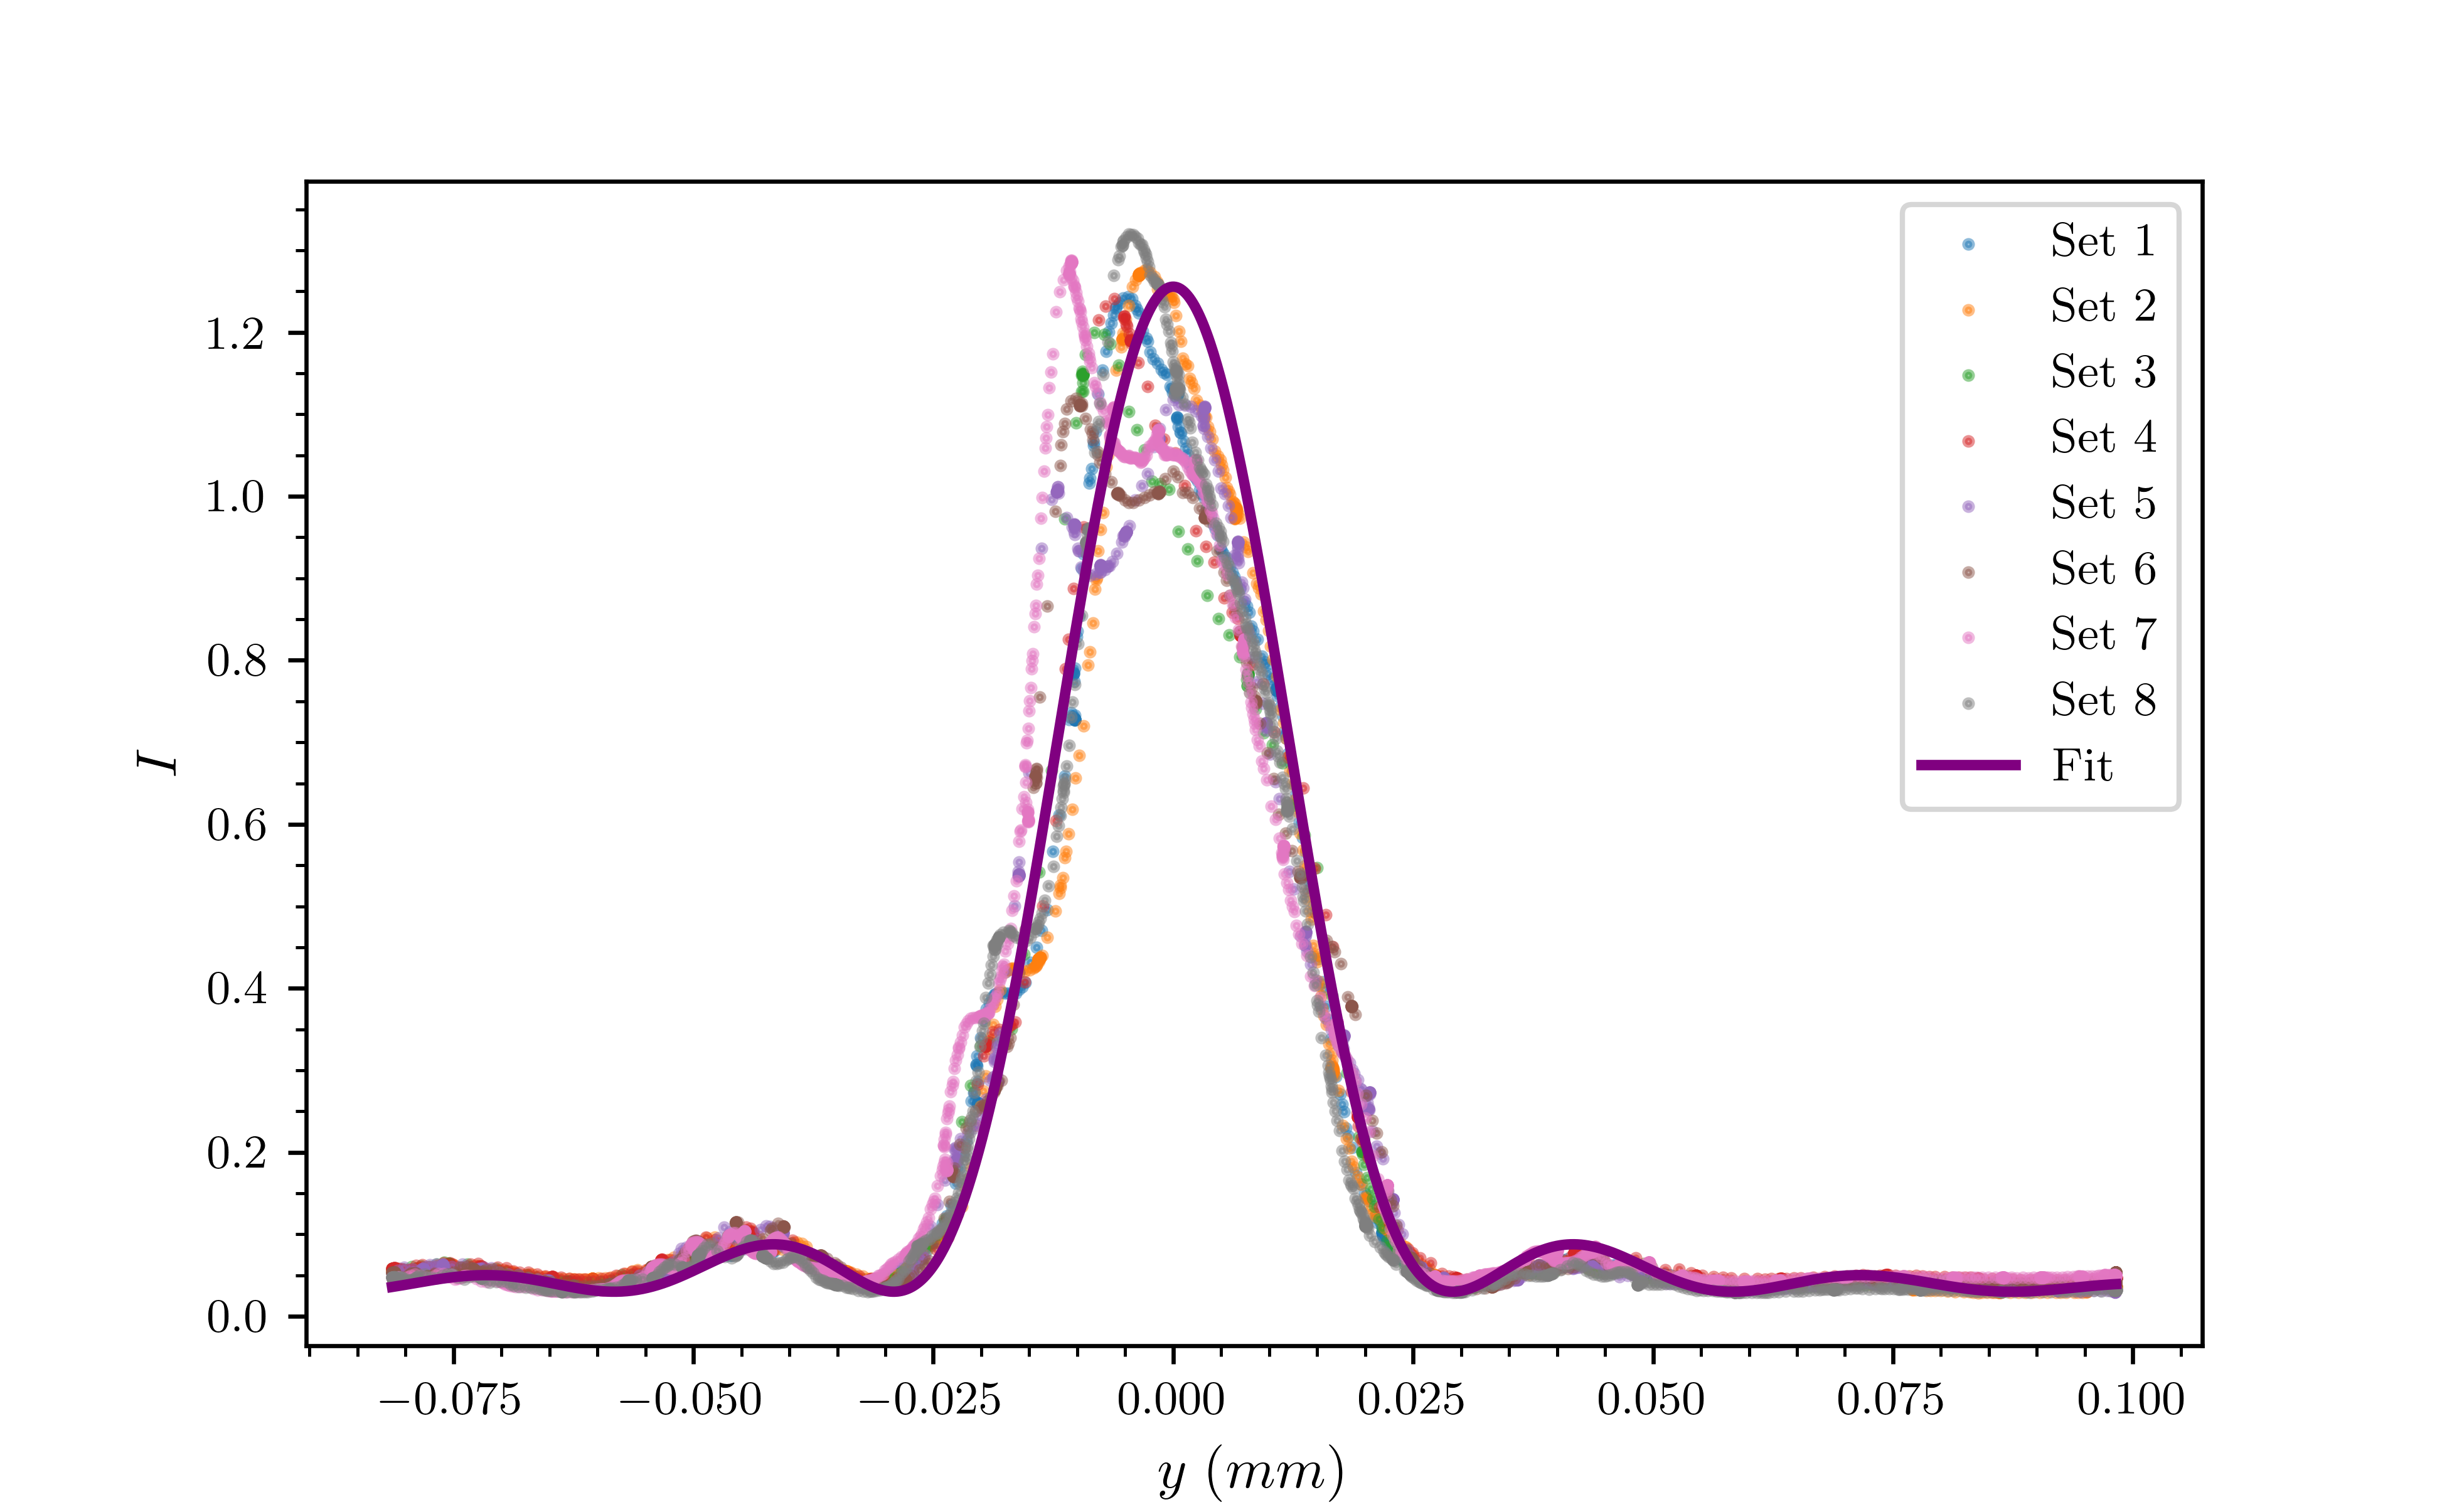
\includegraphics{../graphs/fit_0.02_1.5.png}
%     \caption{Grafico dell’intensità della luce in funzione della posizione (cm). I set riportati sul grafico sono tre, ciascuno riferito ad un’apertura del detector di \num{1.5}, \num{1.0} e \qty{0.5}{\milli\meter}. In questo caso, la fenditura utilizzata è quella da \qty{0.02}{\milli\meter}. Si nota che i dati (in particolar modo quelli situati sul picco) non sono del tutto fedeli al fit.}
%     \label{fig:fit_0.02_1.5}
% \end{figure}

% \begin{figure}[ht!]
%     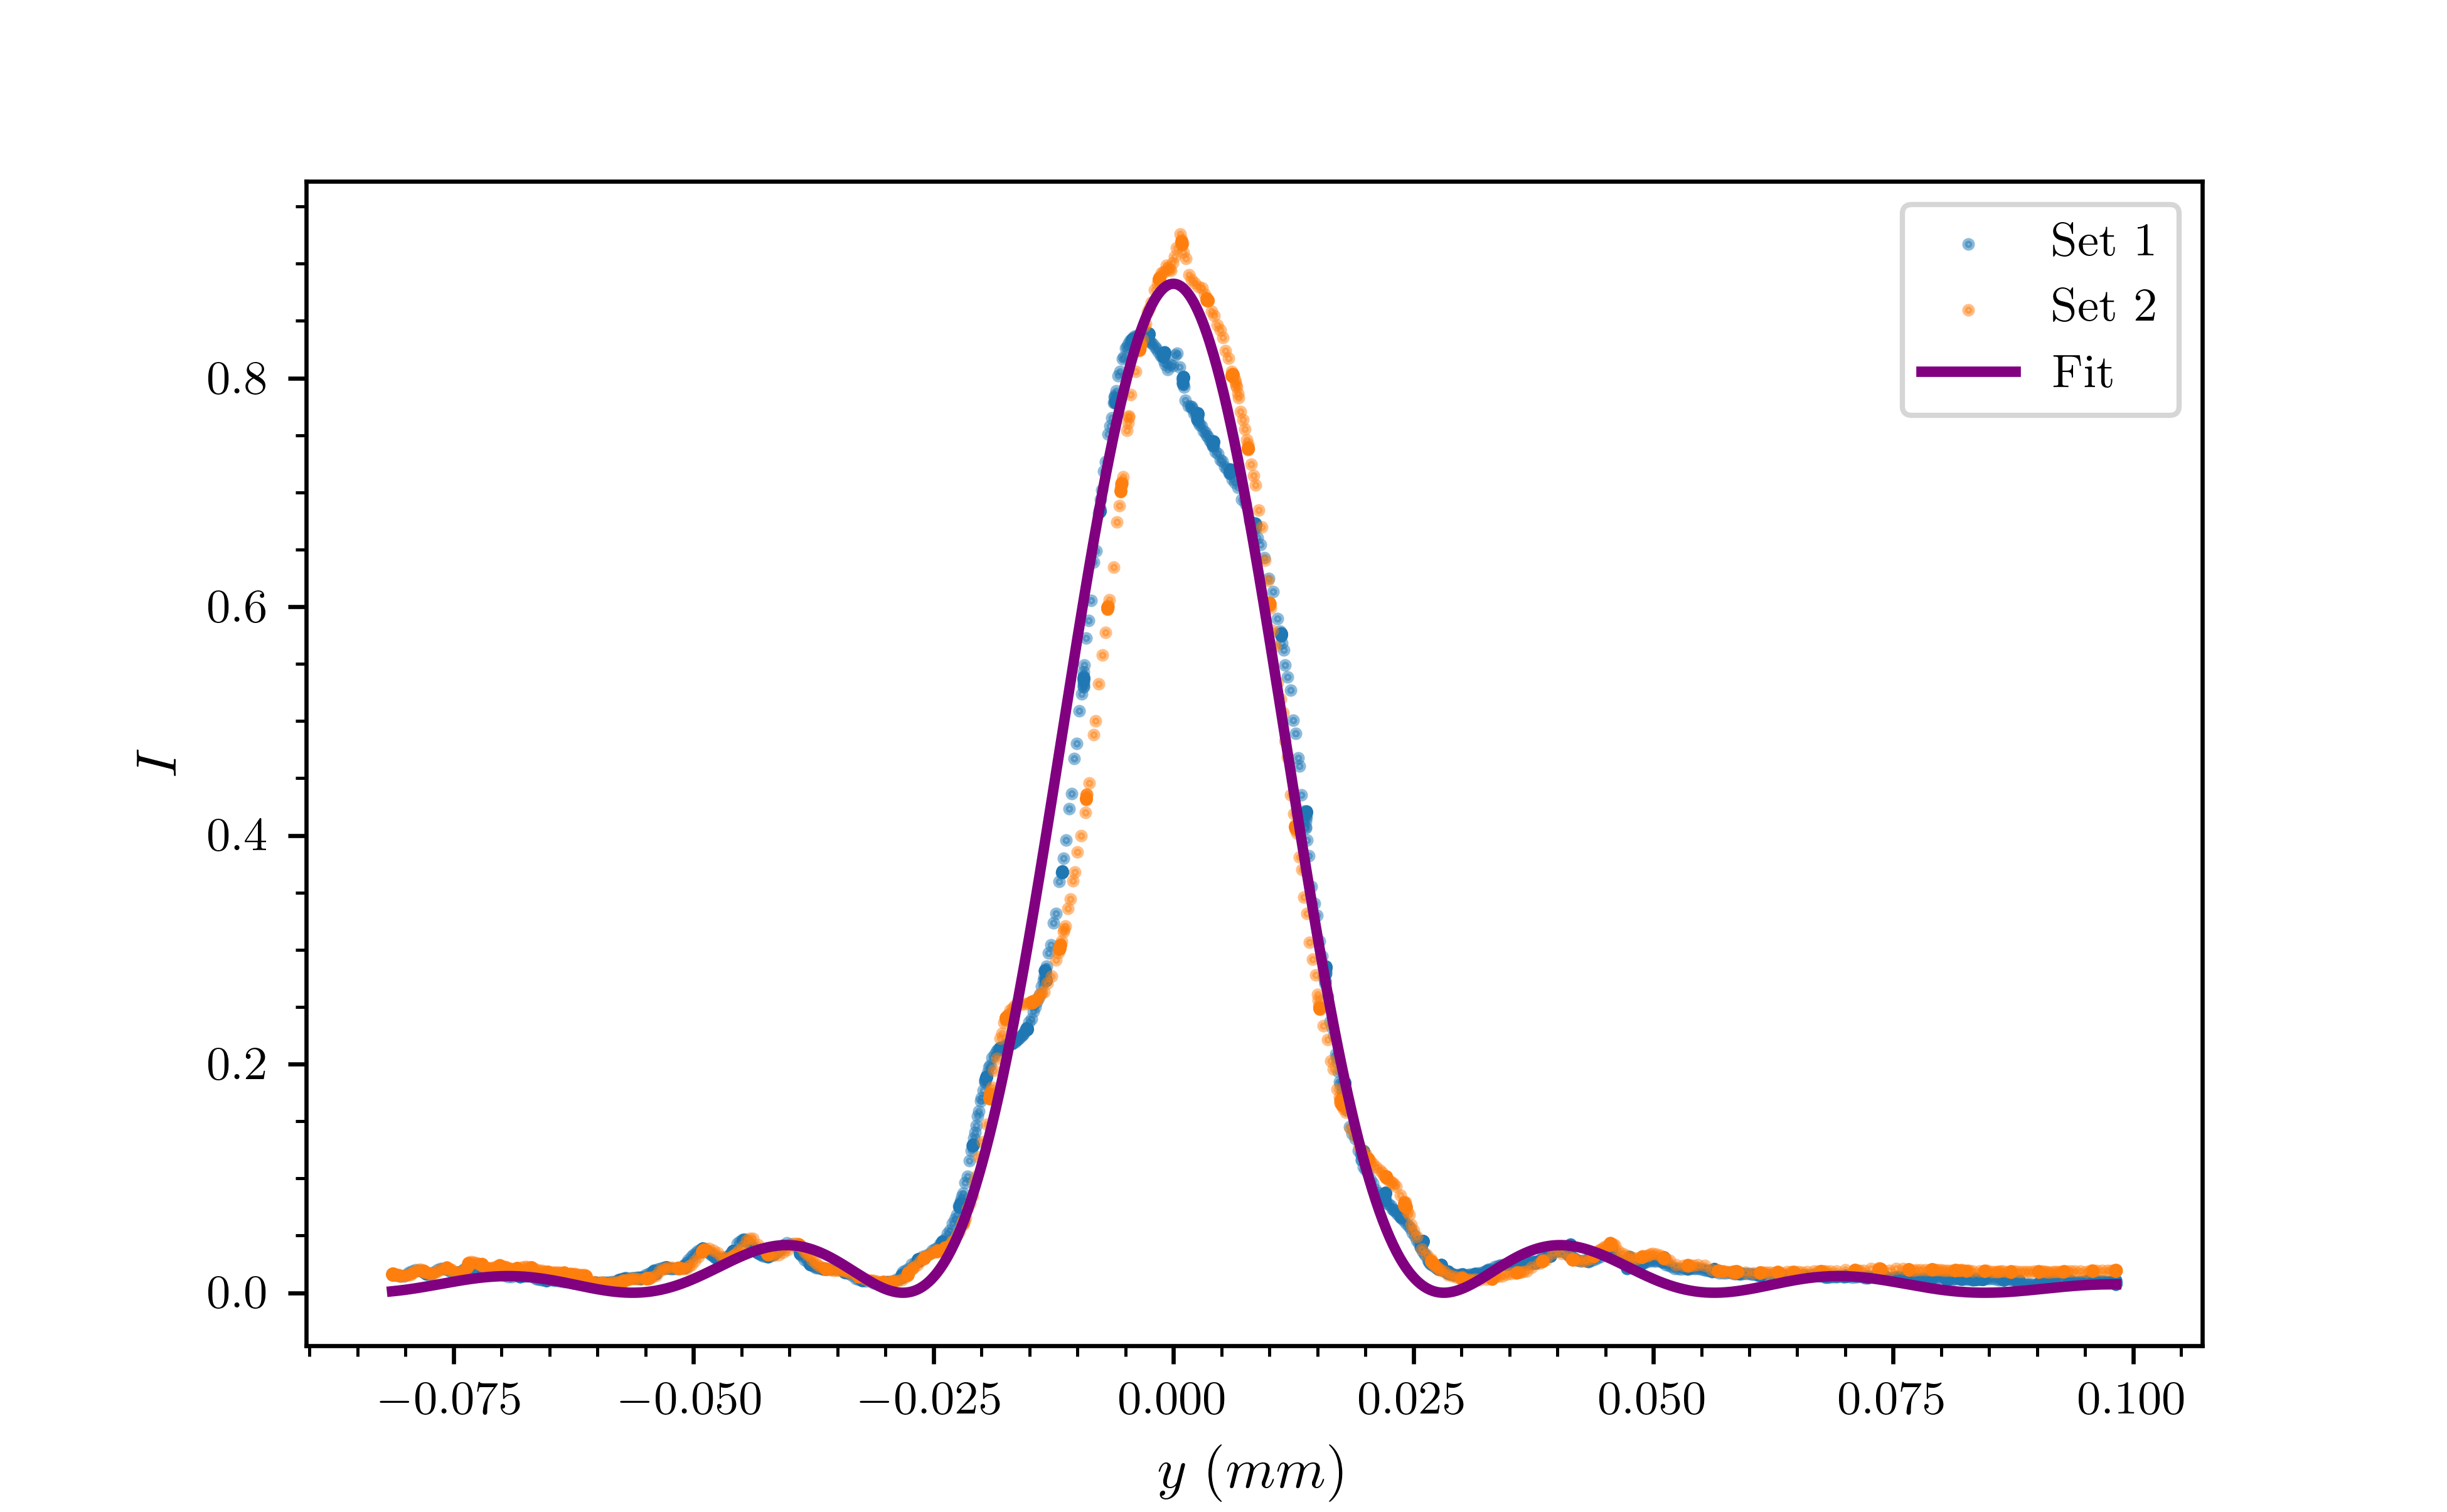
\includegraphics{../graphs/fit_0.02_1.0.png}
%     \caption{}
%     \label{fig:fit_0.02_1.0}
% \end{figure}

% \begin{figure}[ht!]
%     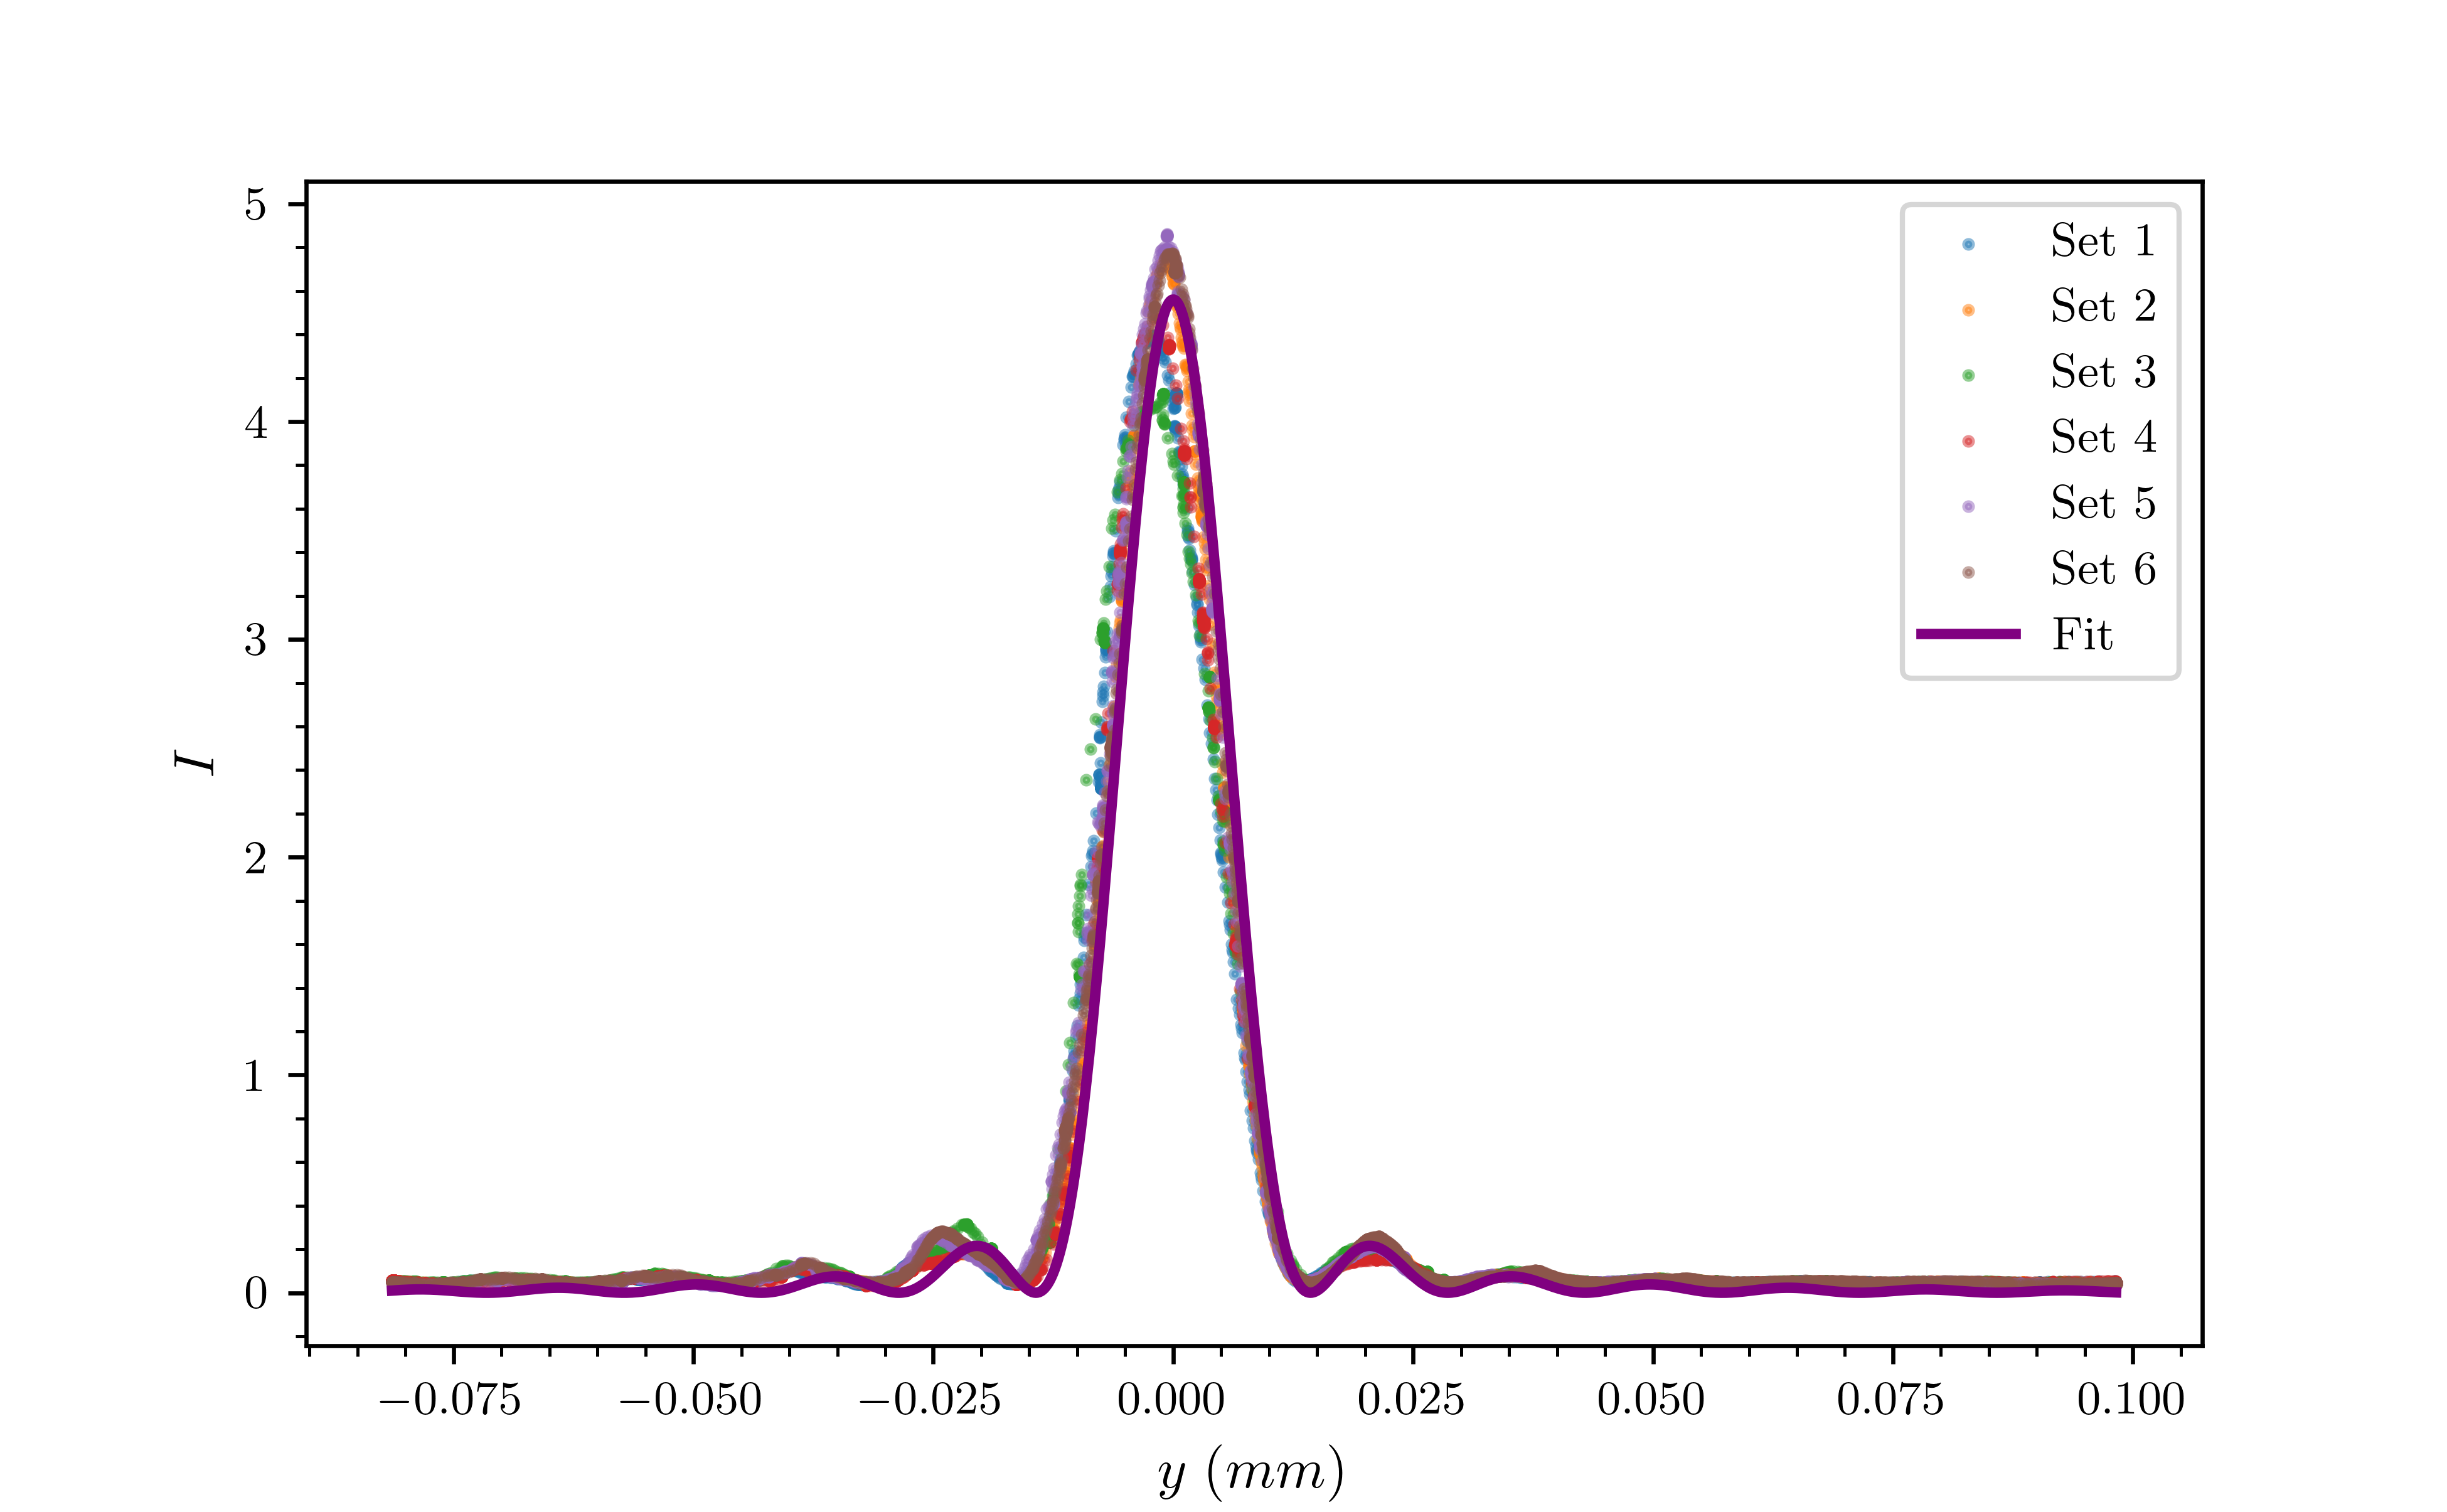
\includegraphics{../graphs/fit_0.04_1.5.png}
%     \caption{Grafico dell’intensità della luce in funzione della posizione (cm). I set riportati sul grafico sono tre, ciascuno riferito ad un’apertura del detector di \num{1.5}, \num{1.0} e \qty{0.5}{\milli\meter}; in questo caso la fenditura utilizzata è quella da \qty{0.04}{\milli\meter}. Qui i dati presentano una migliore fedeltà alla forma del fit, nonostante ci sia un piccolo spostamento verso sinistra.}
%     \label{fig:fit_0.04_1.5}
% \end{figure}

% \begin{figure}[ht!]
%     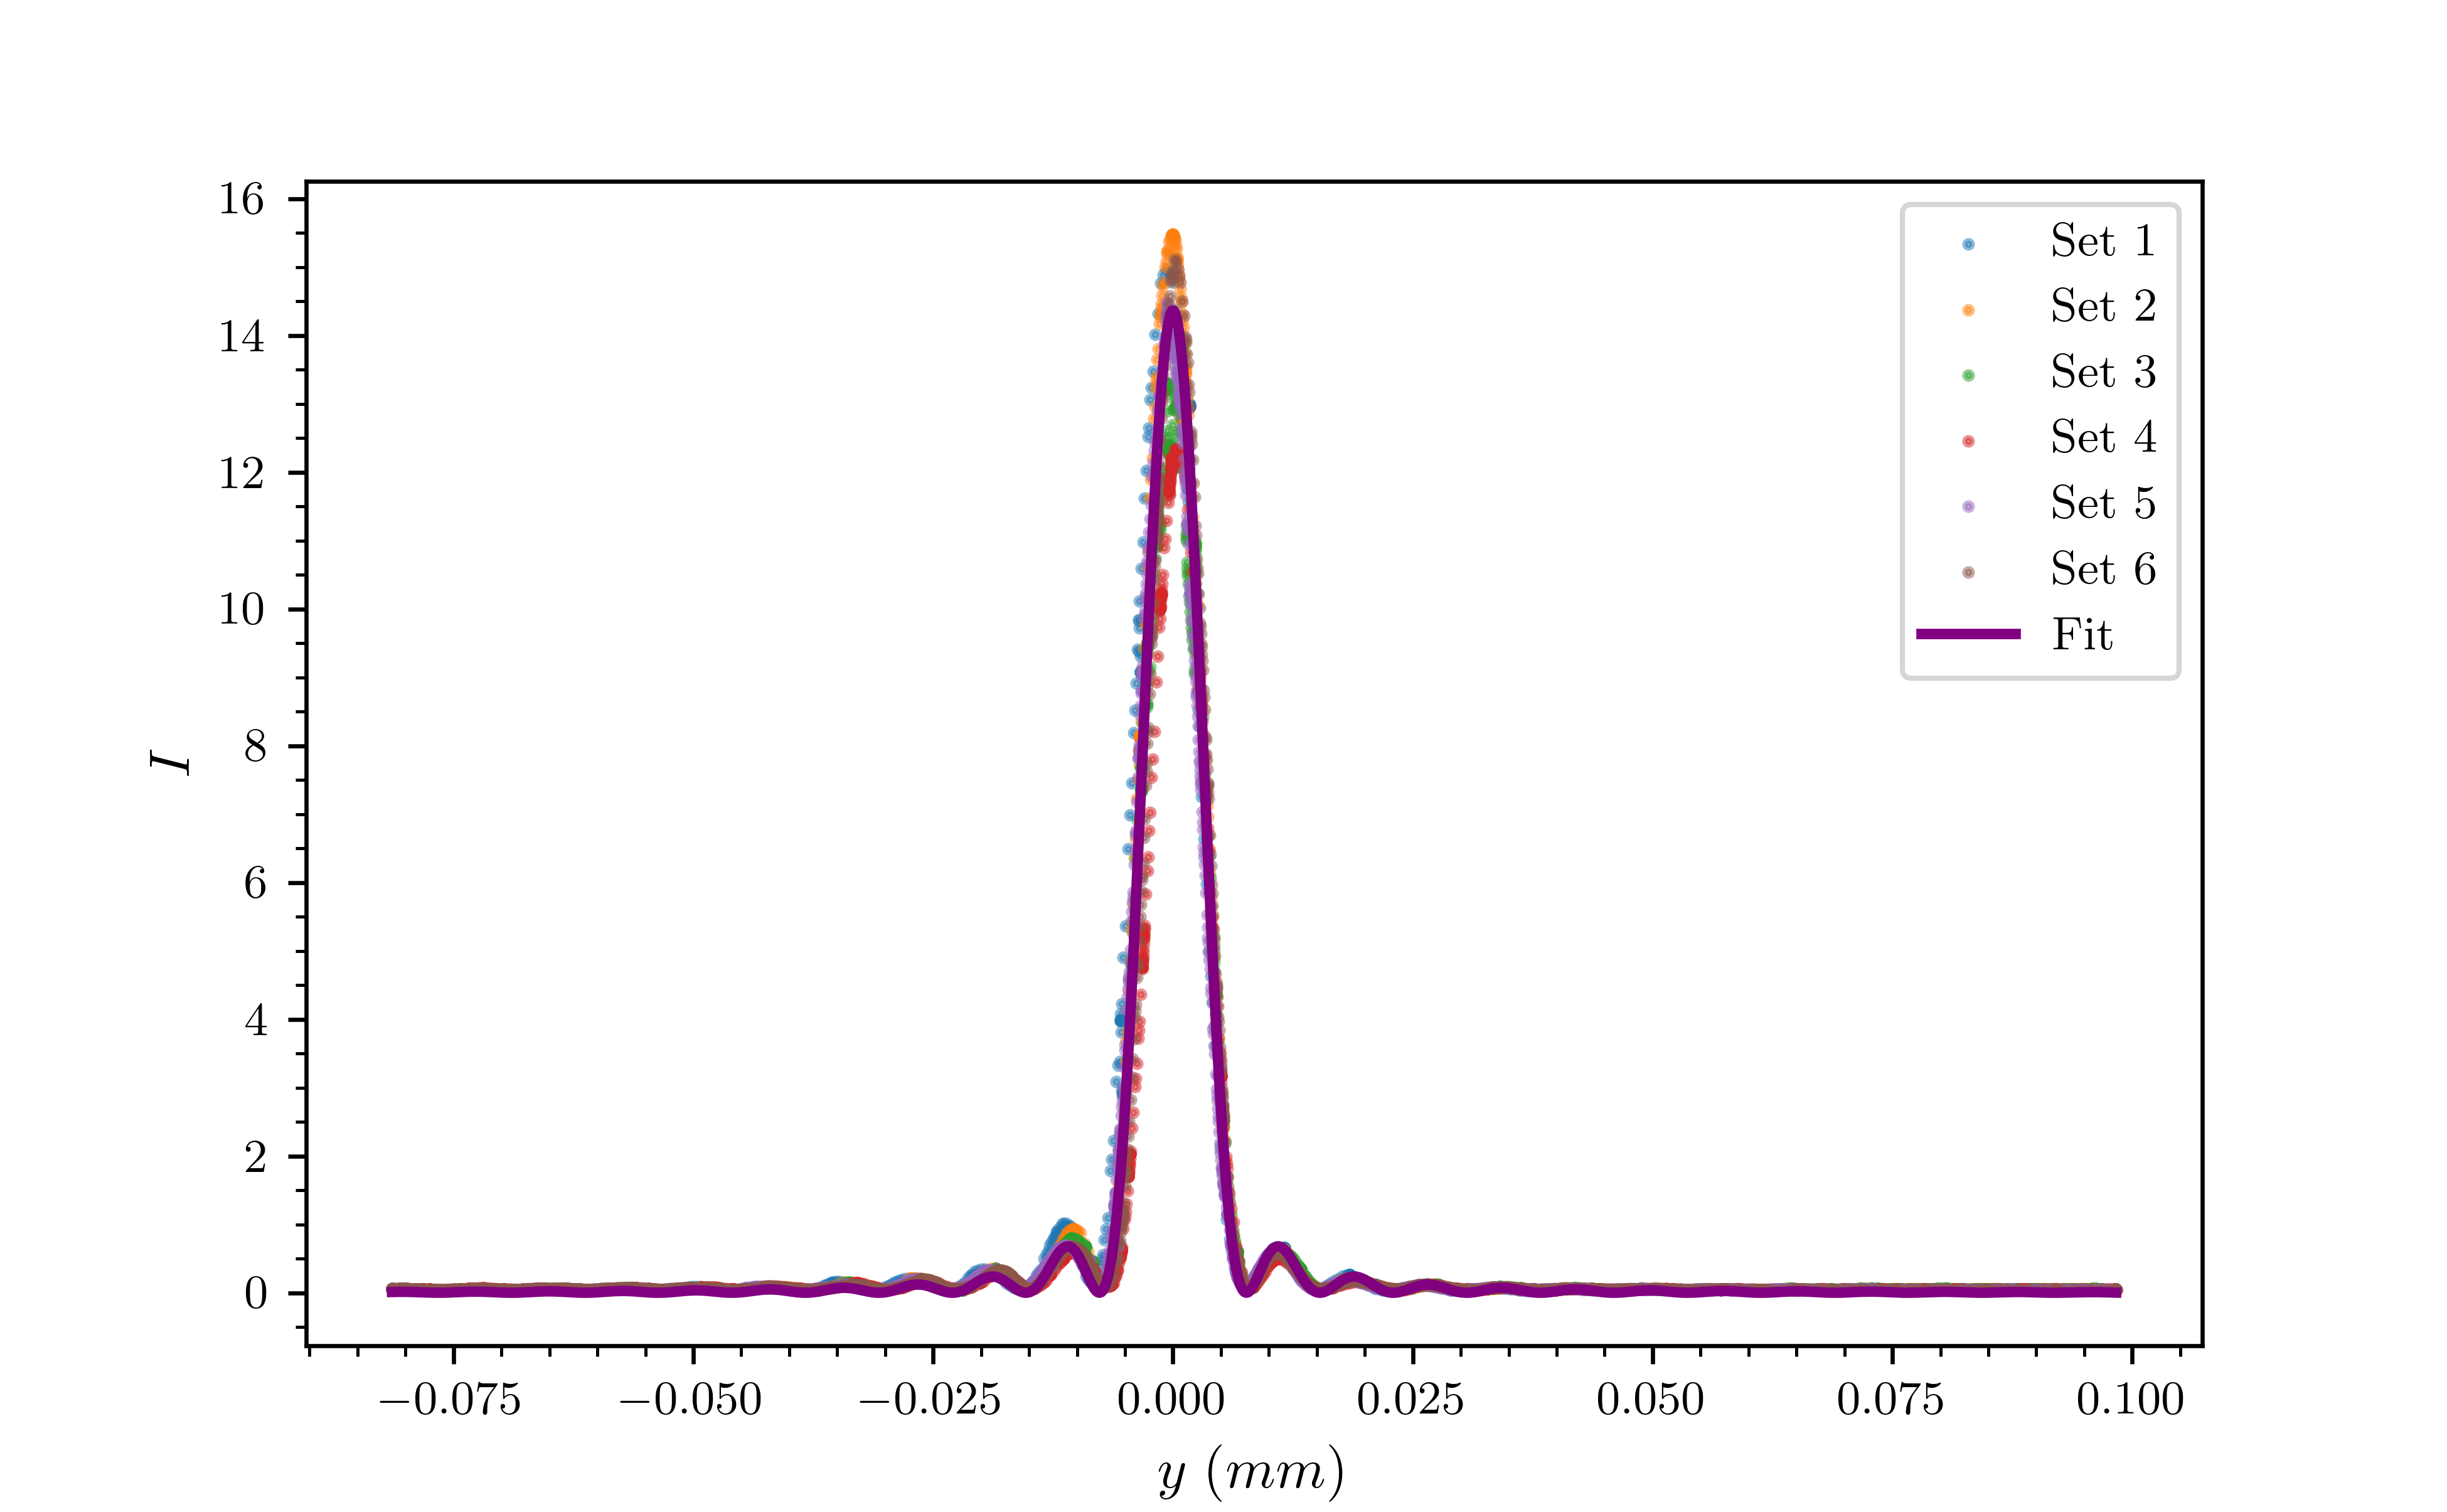
\includegraphics{../graphs/fit_0.08_1.5.png}
%     \caption{Grafico dell’intensità della luce in funzione della posizione (cm). I set riportati sul grafico sono tre, ciascuno riferito ad un’apertura del detector di \num{1.5}, \num{1.0} e \qty{0.5}{\milli\meter}; in questo caso la fenditura utilizzata è quella da \qty{0.08}{\milli\meter}.}
%     \label{fig:fit_0.08_1.5}
% \end{figure}

% %* Stavo per commentare i grafici sopra ma aspetto il "cambio di layout" eventualmente

% Sul grafico seguente, ottenuto come media tra i vari set, si è proceduto a cercare i minimi. Per trovarne la posizione sulle ascisse, sono stati considerati degli intorni centrati sulla posizione teorica di ciascun minimo, data dall'\autoref{eq:y=0 values}, di raggio $\frac{\lambda L}{2 a}$. È bastato infine localizzare il punto di ordinata più bassa in ciascuno di questi intervalli, evidenziati nella (reference alla figura) da rette tratteggiate verticali.

% \begin{figure}[ht!]
%     \includegraphics{../graphs/}
%     \caption{Grafico utilizzato per l'acquisizione dei punti di minimo (punti di interferenza distruttiva).}
%     \label{fig:}
% \end{figure}

\end{document}